% One-page layout: (proof-)reading on display
% \documentclass[11pt,oneside,a4paper]{book}

% Two-page layout: final printing
\documentclass[11pt,twoside,a4paper]{book}   

\usepackage[czech, english]{babel}
\usepackage[T1]{fontenc}
\usepackage[utf8]{inputenc}

\usepackage{graphicx}
% 1. odstavec jako v cestine.
\usepackage{indentfirst} 

% Specialni makra pro formatovani DP a BP.
\usepackage{k336_thesis_macros} 
 
\newcommand\TypeOfWork{Bakalářská práce}  \typeout{Bakalarska prace}
\newcommand\StudProgram{Softwarové technologie a management, Bakalářský}
\newcommand\StudBranch{Softwarové inženýrství}           

\newcommand\WorkTitle{Elektronické volby}
\newcommand\FirstandFamilyName{Tomáš Čerevka}
\newcommand\Supervisor{Ing. Martin Komárek}



% Zvyraznovani odkazu.
%\usepackage[
%pdftitle={\WorkTitle},
%pdfauthor={\FirstandFamilyName},
%bookmarks=true,
%colorlinks=true,
%breaklinks=true,
%rlcolor=blue,
%citecolor=blue,
%linkcolor=blue,
%unicode=true,
%]
%{hyperref}


\usepackage[square, numbers]{natbib} % sazba pouzite literatury
\usepackage[hyphens]{url}
%\DeclareUrlCommand\url{\def\UrlLeft{<}\def\UrlRight{>}\urlstyle{tt}}  %rm/sf/tt
%\renewcommand{\emph}[1]{\textsl{#1}}    % melo by byt kurziva nebo sklonene,
%\let\oldUrl\url
%\renewcommand\url[1]{<\texttt{\oldUrl{#1}}>}

\begin{document}

\selectlanguage{czech}

% prikaz \typeout vypise vyse uvedena nastaveni v prikazovem okne pro pohodlne ladeni prace

\iflanguage{czech}{
	 \typeout{************************************************}
	 \typeout{Zvoleny jazyk: cestina}
	 \typeout{Typ prace: \TypeOfWork}
	 \typeout{Studijni program: \StudProgram}
	 \typeout{Obor: \StudBranch}
	 \typeout{Jmeno: \FirstandFamilyName}
	 \typeout{Nazev prace: \WorkTitle}
	 \typeout{Vedouci prace: \Supervisor}
	 \typeout{***************************************************}
	 \newcommand\Department{Katedra počítačů}
	 \newcommand\Faculty{Fakulta elektrotechnická}
	 \newcommand\University{České vysoké učení technické v Praze}
	 \newcommand\labelSupervisor{Vedoucí práce}
	 \newcommand\labelStudProgram{Studijní program}
	 \newcommand\labelStudBranch{Obor}
}{
	 \typeout{************************************************}
	 \typeout{Language: english}
	 \typeout{Type of Work: \TypeOfWork}
	 \typeout{Study Program: \StudProgram}
	 \typeout{Study Branch: \StudBranch}
	 \typeout{Author: \FirstandFamilyName}
	 \typeout{Title: \WorkTitle}
	 \typeout{Supervisor: \Supervisor}
	 \typeout{***************************************************}
	 \newcommand\Department{Department of Computer Science and Engineering}
	 \newcommand\Faculty{Faculty of Electrical Engineering}
	 \newcommand\University{Czech Technical University in Prague}
	 \newcommand\labelSupervisor{Supervisor}
	 \newcommand\labelStudProgram{Study Programme} 
	 \newcommand\labelStudBranch{Field of Study}
}




% Poznamky ke kompletaci prace
% Nasledujici pasaz uzavrenou v {} ve sve praci samozrejme 
% zakomentujte nebo odstrante. 
% Ve vysledne svazane praci bude nahrazena skutecnym 
% oficialnim zadanim vasi prace.
{
\pagenumbering{roman} \cleardoublepage \thispagestyle{empty}
\chapter*{Zadání}
Na základě existujícího prototypu navrhněte a realizujte systém pro elektronické volby, jehož účelem bude zjednodušení a zrychlení stávajících volebních procesů a kompletní nahrazení \uv{obálkového} hlasování. Systém bude umožňovat hlasování za pomoci dotykových terminálů. Před začátkem hlasování voliči zaregistrují svůj otisk prstu do systému a obdrží číselný PIN. Systém zajistí tajnost a nezfalšovatelnost hlasování. Po ukončení hlasování systém spočítá hlasy a prezentuje výsledky.
\newpage
}

% Titulni stranka

\coverpagestarts

% Podekovani 

\acknowledgements
\noindent
Zde můžete napsat své poděkování, pokud chcete a máte komu děkovat.


%   Prohlaseni 

\declaration{V~Chebu dne 15.\,5.\,2011}
%\declaration{In Kořenovice nad Bečvárkou on May 15, 2008}


% Abstract 
 
\abstractpage

This work deals with the concept and implementation of electronic election system which uses local voting terminals. The system provides easy and quick deployment, secure voting and post-processing results. It also allows the presentation of election results. Main emphasis are security and user-friendly enviroment.

% Prace v cestine musi krome abstraktu v anglictine obsahovat i abstrakt v cestine.
\vglue60mm

\noindent{\Huge \textbf{Abstrakt}}
\vskip 2.75\baselineskip

Tato práce se zabývá návrhem a implementací systému pro správu elektronických voleb za využití lokálních hlasovacích terminálů. Systém zajišťuje snadné a rychlé uvedení do provozu, bezpečné hlasování a následné zpracování výsledků. Zároveň umožňuje prezentaci výsledků voleb. Důraz je kladen na zabezpečení a uživatelskou přívětivost.

% Obsah 

\tableofcontents


% Seznam obrazku 

\listoffigures


% Seznam tabulek

\listoftables


%**************************************************************

\mainbodystarts
% horizontalní mezera mezi dvema odstavci
%\parskip=5pt
%11.12.2008 parskip + tolerance
\normalfont
\parskip=0.2\baselineskip plus 0.2\baselineskip minus 0.1\baselineskip



%*****************************************************************************
\chapter{Úvod}

Na schůzích a zasedáních dochází často k rozhodování mezi několika možnostmi. Může se jednat o zvolení kandidáta do funkce, nebo se může například hlasovat o nepersonálních otázkách\footnote{Například využití peněz z fondu, kudy povede nová dálnice, jak vyřešit stávku etc.}. Jelikož ne všichni jsou vždy stejného názoru a je třeba rozhodnout kolektivně, přistupuje se k hlasování. Hlasování může být veřejné, tj. ví se, jak kdo hlasoval, nebo tajné, kdy je každý hlas anonymní. V obou případech je ovšem třeba zajistit, aby mohly hlasovat jen k tomu oprávněné osoby.

Tématika elektronických voleb je poslední dobou stále častěji zmiňována v souvislosti s rozvojem moderních technologií a internetu. Modernizace stávajícího volebního systému je základním pilířem tzv. systému elektronického vlády, e-governmentu. Přínosy elektronického hlasování jsou podrobně popsány v kapitole \ref{sec:motivace}, ale ruku v ruce s nimi jde i řada technických a organizačních otázek, které je třeba řešit a jejichž základní nástin nabízí kapitola \ref{sec:bezpecnostni_rizika}.

Cílem této práce je jejich zodpovězení a vytvoření funkčního systému, který umožní realizovat elektronické volby za pomoci dotykových terminálů ve volební místnosti. Centrální server bude od terminálů přijímat jednotlivé hlasy a na konci hlasování prezentuje výsledky.


%*****************************************************************************
\chapter{Popis problému, specifikace cíle}

\section{Motivace} \label{sec:motivace}

V současné době probíhá většina voleb bez jakéhokoliv elektronického systému. Při veřejném hlasování voliči pouze zvednou ruku a pověřená osoba je spočítá. Tajné volby bývají realizovány za pomoci volební urny a obálek. Na začátku se každý volič prokáže osobním dokladem, obdrží orazítkovanou volební obálku s volebními lístky a vydá se za plentu, kde z volebních lístků jeden vybere, vloží ho do obálky a tu následně vhodí do urny. Když takto odhlasují všichni, pověřená osoba urnu rozpečetí a ručně sečte všechny hlasy. Na obrázku \ref{fig:soucasny_stav} je diagram aktivit znázorňující průběh voleb bez elektronického systému.

\begin{figure}[h]
	\centering
	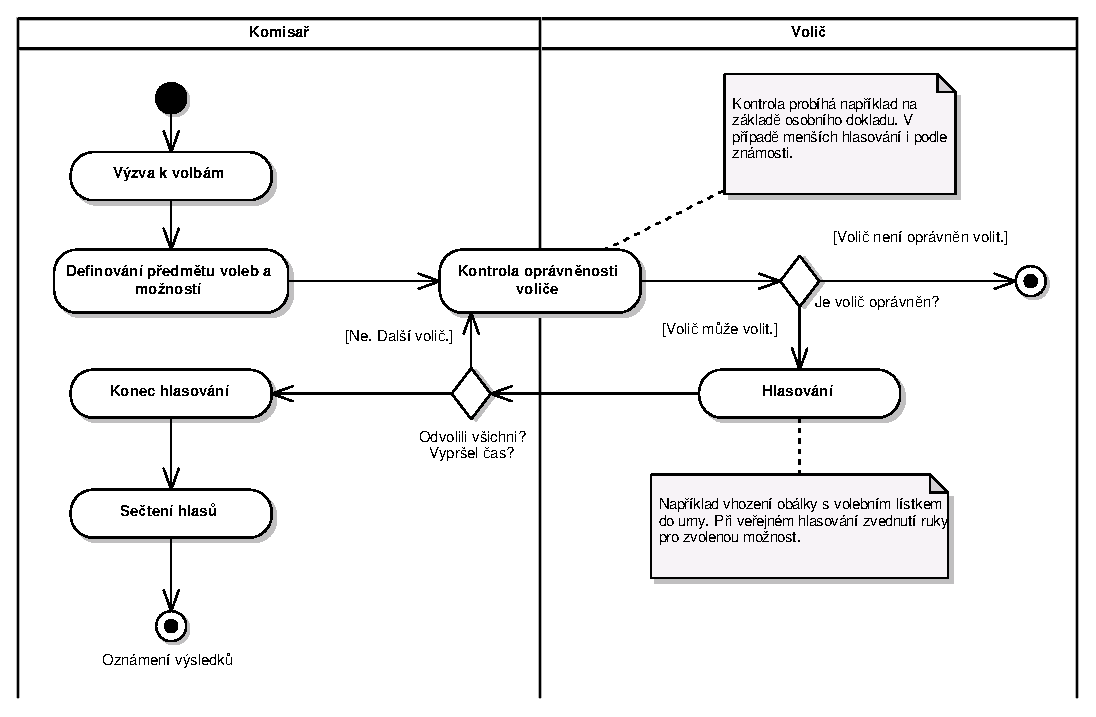
\includegraphics[scale=0.9]{diagrams/soucasny_stav.eps}
	\caption{Diagram aktivit voleb bez elektronického systému.}
	\label{fig:soucasny_stav}
\end{figure}

Tento způsob voleb je sice funkční a léty prověřený, ovšem jeho realizace je časově a personálně náročná na přípravu, na samotný průběh voleb a následné sčítání hlasů. Jeho slabinou je možnost selhání lidského faktoru, na kterém je tento proces příliš závislý. To by mohlo zapříčinit jak neúmyslné chyby, tak zcela cílevědomé ovlivnění výsledků.

\section{Rešerše} 

Elektronické volby jsou tématem, které již bylo mnohokrát zpracováváno. Následující odstavce rozebírají několik zdrojů, ze kterých tato práce vychází, a stručně popisují jejich obsah.

\subsection{Prototyp systému eVolby}

Implementační část této bakalářské práce vychází z prototypu systému internetových elektronických voleb pro Akademický senát ČVUT, který vznikl v rámci předmětů Y36SI2 a Y36SI3 \cite{www:prototyp}. Tento systém se sestává pouze ze serveru napsaném v Enterprise Javě, který zajišťuje jak administraci voleb, tak samotné hlasování voličů přes internet. 

Prototyp je koncipován pouze pro personální volby, kdy se nejprve z řad voličů nominují kandidáti. Po ukončení nominací následuje hlasování, kdy voliči dávají své hlasy jednotlivým kandidátům. V této práci bude systém rozšířen o možnost i nepersonálních voleb, kdy předmět voleb a možnosti budou definovány explicitně při jejich zakládání.

V systému figurují tři role uživatelů: administrátor, komisař a volič. Pro lepší správu kandidátů přidává nový koncept další uživatelskou roli: kandidáta. Administrátor je v systému pouze jeden a má pravomoc založit volby a jmenovat jim komisaře. Jedny volby mohou mít více komisařů a v případě důležitého rozhodnutí je třeba potvrzení alespoň nadpoloviční většiny. Komisaři pod volbami zakládají volební události představující jednotlivá kola voleb. K těm přiřazují oprávněné voliče a schvalují či vyřazují nominované kandidáty.

\subsection{Experimentální ověření distribuovaného volebního schématu}
Konceptuální návrh podobného systému zpracoval ve své disertační práci \textit{Experimentální ověření distribuovaného
volebního schématu} Radek Šilhavý \cite{art:silhavy}. Tato práce se zabývá hlavně teoretickou rovinou a popisu procesů a požadavků na realizaci elektronických volebních systémů a dává k dispozici ucelený pohled na problematiku. Důraz je kladen hlavně na internetové volební systémy umožňující vzdálené hlasování bez nutnosti fyzické účasti ve volební místnosti.

V úvodu se autor zabývá teoretických rámcem od legislativní problematiky v prostředí České republiky až po praktické využití ve světě. Popisuje, v jaké podobě byly elektronické volby testovány nasazovány ve Spojených státech amerických, Německu, Velké Británii, Španělsku, Švýcarsku a Estonsku.

Zbytek práce se již orientuje více prakticky na návrh konceptuálního řešení distribuovaného volebního schématu a stanovuje hypotézy pro experimentální ověření hypotéz. První hypotéza předpokládá, že elektronizace volebního procesu za využití internetového volebního systému je možná a že je přínosem pro voliče. Druhá hypotéza prohlašuje využití webové aplikace jako základního řešení za výhodné, protože každému uživateli je přístupná a dostupná v čase a místě jemu vyhovujícím.

\subsection{Hlasovací systém pro samosprávné orgány vysokých škol}
Problematikou elektronických voleb se zabývá i diplomová práce Michala Petříka \textit{Hlasovací systém pro samosprávné orgány vysokých škol} \cite{art:petrik}. Zde se autor zaměřuje hlavně na potřeby samosprávných orgánů vysokých škol, speciálního Akademického senátu FIT ČVUT. 

Tento systém je navržen tak, aby dokázal zautomatizovat online hlasování, správu jednotlivých hlasování v rámci zasedání, generování usnesení ze zasedání a prezentaci vybraných informací na webové stránky. Je zde propracován systém oprávnění, který umožňuje přidělovat libovolná administrátorská práva uživateli nebo skupině uživatelů. Autentizace uživatelů je velmi rozsáhlá, neboť poskytuje několik různých cest: přes uživatelské účty v databázi LDAP, pomocí identifikační karty či samotným systémem. 

\subsection{Mobilního hlasovacího zařízení}

Hlavním účelem elektronických voleb je snaha o zpříjemnění a zrychlení práce se samotnými hlasy. Proto je také důležité zpracování terminálového klienta, který si za vzor bere \textit{Mobilní hlasovací zařízení} \cite{art:valenta} Jakuba Valenty. Autor se sice zabývá problematikou hlasovacího zařízení v podobě mobilního telefonu s technologií Wi-Fi, ale podobnost s terminálovým klientem z hlediska analýzy je značná. Kromě toho rozebírá síťovou komunikaci posíláním zpráv v jazyce XML přes protokol HTTP.

Na implementaci je zajímavá vícevrstvá architektura dělená na prezentační, aplikační, datová, persistentní a síťovou vrstvu. Serverová část v sobě také zahrnuje modul pro generování výsledků, jehož studium v sobě skrývá potenciál využitelný při zpracovávání hlasů a prezentaci výsledků.

\subsection{Rešerše algoritmů pro snímání a zpracování otisku prstů} \label{sec:reserse_otisky}

Při volbách se voliči budou přihlašovat za pomoci otisku prstu a PINu. Pro tyto účely je pro třeba zvolit správnou čtečku otisků prstů, která zajistí spolehlivost, dlouhou životnost a cenovou dostupnost. \textit{Rešerše algoritmů pro snímání a zpracování otisku prstů} \cite{art:polackova} od Zuzany Poláčkové poskytuje podrobný náhled do oblasti daktyloskopie. Kromě jiného pojednává o základních biometrických systémech, zpracování otisků prstů a o algoritmech používaných v praxi. Nejdůležitější je pro mě kapitola o snímačích otisků prstů, kde porovnává výhody a nevýhody optoelektrických, kapacitních, teplotních, elektroluminiscenčních a ultrazvukových snímačů.

Jako nejlepší volba se jeví elektroluminiscenční snímač, jelikož pořizuje kvalitní výstup v digitální podobě, nemá problémy se snímáním extrémně suché pokožky a je cenově dostupný. Mezi nevýhody sice patří menší odolnost a citlivost na prach a vodu, ale oproti ostatním snímačům je to zanedbatelné.

\subsection{Electronic Voting in Europe - Technology, Law, Politics and Society}

Ve dnech 7. a 9. července 2004 se konal první mezinárodní workshop \textit{Electronic Voting in Europe - Technology, Law, Politics and Society} \cite{book:prosser} v Schloß Hofenenu v Rakousku. Z tohoto workshopu vznikla stejnojmenná kniha v podobě sborníku prací. Kniha rozebírá problematiku elektronických voleb ze všech možných úhlů a představuje systémy používané v Evropě. Dotýká se témat bezpečnosti, hrozících rizik a jejich řešení, biometrických systémů, technických požadavků a legislativních principů.

\subsection{Elektronické volby u nás a ve světě}

Na portále \texttt{www.internetprovsechny.cz} vyšel rozsáhlý článek \cite{www:estonsko} pojednávající o elektronických volbách v Estonsku. Estonsko je pokládáno za internetově velmi vyspělou zemi. Už jen skutečnost, že jejich ústava zaručuje od roku 2000 všem jejich občanům přístup na internet je toho dostatečným důkazem.

Důležitou skutečností, která výrazně pomohla zavedení elektronických voleb, bylo zavedení elektronických identifikačních průkazů\footnote{Obdoba našich občanských průkazů.}. ID karta obsahuje nejen strojově čitelný kód, ale i mikročip, který má na sobě uloženy dva digitální certifikáty a související privátní klíče chráněné PIN kódy. Jeden certifikát slouží k autentizaci, druhý k elektrickému podpisu, přičemž je každý může používat bez omezení. Nejsou tedy vázány jen na komunikaci se státem.

Zajímavostí modelu hlasování je zabezpečení hlasů. Funguje na tzv. principu dvou obálek. Hlasovací lístek se zašifruje klíčem voleb, což tvoří vnitřní obálku. Vnější obálku představuje elektronický podpis vnitřní obálky. Díky tomuto systému je možné, aby hlas nebyl spojen s voličem, ale zároveň volič může hlasovat vícekrát, kdy se započítá jen poslední hlas. Tento koncept byl zvolen kvůli eliminaci hlasování pod tlakem. U klasických voleb přistupuje volič za plentu samostatně, ovšem u voleb přes internet nelze zajistit jeho soukromí. Kdyby někdo voliče nutil hlasovat jinak, než on sám chce, může tak učinit, ale pak svůj hlas může změnit.

Portál \texttt{www.lupa.cz} \cite{www:lupa} uveřejnil článek, který se více orientuje na situaci v tuzemsku. Nejdříve ovšem popisuje výhody a nevýhody elektronických voleb a zkušenosti v zahraničí, načež informuje o tom, že ČSÚ je již přepraven na jejich modernizaci \cite{www:csu}. 

\section{Požadavky}

\subsection{Nefunkční požadavky}

V této sekci jsou stanoveny požadavky, které se netýkají funkčnosti, nýbrž jsou kladeny na celkový návrh, použité technologie a zpracování.

\subsubsection{Obecné požadavky} \label{sec:obecne_pozadavky}

Na celkový návrh řešení a dokumentaci jsou kladeny následující požadavky:

\begin{enumerate}
	\item Systém bude rozdělen na serverovou a klientskou část.
	\item Instalace systému a jeho uvedení do provozu bude co nejjednodušší a nejrychlejší.
	\item Systém bude multiplatformní díky běhovému prostředí JVM.
	\item Systém bude používat open source nebo freeware technologie.
	\item Systém zajistí bezpečnost hlasování, tj. nezfalšovatelnost hlasů a tajnost voleb vůči druhé i třetí osobě.
	\item Součástí systému bude podrobná dokumentace.
\end{enumerate}

\subsubsection{Server}

Serverová část aplikace řídí celý průběh voleb, zpracovává požadavky od klientů a poskytuje jim data. Server:

\begin{enumerate}
	\item zajistí práci s databází a validaci dat.
	\item definuje rozhraní klientským aplikacím.
	\item bude využívat technologii Java EE.
\end{enumerate}

\subsubsection{Terminálový klient}

Samostatná aplikace běžící na dotykovém terminálu, která umožňuje hlasování. Vyžaduje připojení k serverové části aplikace. Klient:

\begin{enumerate}
	\item umožní voličům hlasovat.
	\item umožní voličům registraci.
	\item si neukládá žádná data. Vše předává přes protokol HTTPS serverové části. 
	\item bude používat technologii Java SE a Java FX.
\end{enumerate}

\subsection{Funkční požadavky}

Tato sekce se zabývá požadavky na funkčnost systému. Systém umožní:

\begin{enumerate}
	\item založení voleb.
	\item založení volební události.
	\item přiřazení komisaře k volbám.
	\item registrace voliče.
	\item přiřazení voličů k volební události.
	\item nominování kandidátů.
	\item hlasování.
	\item prezentaci výsledků.
\end{enumerate}

\section{Fáze elektronických voleb}

Životní cyklus voleb je neměnný a čítá několik fází, které je třeba důkladně ošetřit. Pro zvýšení efektivity práce se systémem je třeba průběh každé fáze co nejvíce uživatelsky zjednodušit.

\subsection{Registrace voličů}

Před zahájením voleb je třeba do systému zanést seznam voličů s jejich nacionáliemi, kteří jsou oprávněni se zaregistrovat. Díky tomuto opatření se minimalizuje riziko, že se do voleb zaregistruje neoprávněná osoba a zároveň bude evidováno, kteří voliči se k registraci ještě nedostavili. Tato skutečnost může být důležitá pro volby, kdy je třeba přítomnost pevně dané části voličů, aby volby byly usnášeníschopné.  

Na průběh registrace voličů bude dohlížet pověřená osoba, která bude voliče připouštět k registraci po kontrole dokladu totožnosti, přičemž vždy na příslušném registračním terminálu vyvolá registraci voliče z předdefinovaného seznamu.

Registrace bude obnášet sejmutí otisku prstu a vygenerování přístupového PINu. Otisk prstu zabrání případnému hlasování v zastoupení, kdy by volič sdělil svůj PIN neoprávněné osobě. PIN slouží jako druhotný autentizační prvek, který vyloučí případnou chybu čtečky otisků prstů. 

\subsubsection{Seznamy voličů} \label{sec:seznamy}

Dá se předpokládat, že systém bude používán na více než jedny volby, přičemž seznam voličů se mezi jednotlivými volbami bude lišit jen minimálně, ne-li vůbec. Správce voleb si tedy může jednotlivé voliče zařadit do seznamu, přičemž jeden volič může být obsažen ve více seznamech, ovšem nemusí být v žádném. Při zakládání hlasování pak může voliče přidávat jednotlivě nebo hromadně naimportovat celé seznamy voličů bez ohledu na to, zda již jsou v systému zaregistrování, nebo jejich předpřipravené účty zatím na registraci čekají.

\subsection{Založení voleb}

Když jsou v systému připraveni uživatelé, ať již zaregistrovaní či nezaregistrovaní, musí se založit volby. To učiní administrátor a deleguje volbám komisaře z databáze uživatelů. Komisař může být zároveň volič, ale nemusí jím být. Systém předpokládá, že jedny volby mohou mít více kol. Proto komisař pod volbami založí volební událost, ke které přiřadí oprávněné voliče\footnote{Viz. kapitola \ref{sec:seznamy}} a nastaví detaily voleb. Jedná-li se o volby personální, následují nominace popsané v kapitole \ref{sec:nominace}. U voleb nepersonálních je tato fáze vynechána a komisaři nadefinují možnosti hlasování explicitně. Poté zahájí hlasování. Pokud je k daným volbám přiřazeno více komisařů, je pro zahájení hlasování třeba potvrzení alespoň nadpoloviční většiny z nich.

\subsection{Nominace} \label{sec:nominace}

Nominace se týkají pouze voleb personálních a jsou zahajovány alespoň nadpoloviční většinou komisařů. V této fázi se může volič nominovat a stát se tak zároveň kandidátem. Součástí kandidatury je kandidátní listina s volebním programem a fotografií kandidáta. Kandidát má možnost kandidátní listinu upravovat nebo svou kandidaturu zrušit, dokud nejsou nominace ukončeny. Komisaři mají právo kandidáta do systému zadat ručně nebo kandidaturu zrušit. Pro ukončení nominací je třeba souhlas alespoň nadpoloviční většiny komisařů. 

\subsection{Hlasování}

K hlasování voliči používají terminálového klienta, za jeho pomoci se identifikují otiskem prstu a následně se autentizují svým PINem. Systém si nechá potvrdit voličovu totožnost a zobrazí mu předmět voleb s možnostmi, pro které může hlasovat. Volič odhlasuje a jeho volební lístek se odešle ke zpracování na server. Server hlas uloží bez informace, komu patří, a u voliče si nastaví příznak, že již odhlasoval.

\subsection{Výsledky}

Hlasování ukončuje komisař, v případě více komisařů nadpoloviční většina z nich. Celé volby uzavírá administrátor, pokud jsou všechna hlasování v nich ukončena. Systém zpracuje hlasy a vyhodnotí výsledky.

\section{Bezpečnostní rizika} \label{sec:bezpecnostni_rizika}

Jak již bylo zmíněno v kapitole \ref{sec:motivace}, volby jsou provázeny mnoha faktory, které mohou nepříznivě ovlivnit jejich výsledky. Elektronická verze hlasování potlačuje do pozadí lidský faktor a minimalizuje tak jeho negativní dopad, ovšem objevují se nové hrozby, jejichž dopad by mohl být mnohem horší. Těm se ale můžeme efektivně bránit.

\subsection{Hrozby}

Hrozby se dají obecně rozdělit do dvou kategorií: 

\begin{itemize}
	\item manipulační
	\item sabotující
\end{itemize}	

Ke zmanipulování voleb může dojít ze strany komisaře, který využije svých práv v systému a upraví výsledky, nebo ze strany voliče, který se pokusí hlasovat vícekrát, případně hlasovat cizím jménem. Výsledky mohou také být ovlivněny hackerským útokem modifikujícím hlasy. Všechny tyto snahy o manipulaci s daty se snaží nevzbudit žádné podezření a zůstat tak neodhaleny. 

Na druhé straně jsou hrozby, které mohou zabránit průběhu hlasování. Ty se dají dále dělit na úmyslné a neúmyslné. Mezi neúmyslné může například patřit přerušení dodávky elektřiny, či selhání hlasovacího systému vinou neodhalené chyby. Naopak mezi úmyslné hrozby patří DDoS útok \cite{www:ddos} na server, úmyslné přerušení dodávky elektřiny či neoprávněná manipulace s hardwarem a softwarem.

\subsection{Zabezpečení}

U voleb musí byt zajištěno nezfalšování hlasů, proto je třeba, aby všechny volební terminály komunikovaly se serverem pomocí protokolu HTTPS a veškerá komunikace mezi nimi byla zašifrovaná. Dále je třeba zajistit, aby volba každého voliče byla tajná. Toho se docílí neevidování vazby mezi hlasem a voličem. Jakmile tedy volič odhlasuje, přičte se ke zvolené možnosti hlas, systém si uloží, že tento volič již hlasoval, a znemožní mu další hlasování v daném kole voleb.

%*****************************************************************************
\chapter{Analýza}

\section{Uživatelské role}

Volební procesu se účastní mnoho osob, které se dělí do rolí, které při volbách představují. Pro snazší orientaci uvádím jejich výčet.

\subsection{Administrátor}

Úkolem administrátora je zakládání a ukončování voleb a jmenování komisařů. Na samotný průběh voleb nemá žádný vliv. 

\subsection{Komisař}

Komisař je jmenován administrátorem a je přiřazen k volbám. Komisařů pro jedny volby můžu být více, pak v důležitých momentech voleb rozhoduje nadpoloviční většina z nich. Komisař zakládá v rámci voleb jednotlivé volební události, definuje jejich nastavení a přiřazuje k nim oprávněné voliče. Jeho úkolem je zahajování a ukončování nominací a hlasování.

\subsection{Volič}

Volič modifikuje a odevzdává volební lístek ve volbách, ve kterých je oprávněn hlasovat. Také se může nominovat na kandidáta.


\subsection{Kandidát}

Kandidát je nominovaný volič a může být zvolen. Má možnost upravovat svou kandidátní listinu a stáhnout kandidátku, dokud jsou volby ve fázi nominací.

\section{Případy užití}

Případy užití jsou částečně popsané v předchozích kapitolách. Pro úplnost je na obrázku \ref{fig:pripady_uziti} znázorněn use case diagram. Oproti předchozím kapitolám jsou na něm zachyceny i systémové role v podobě uživatelů \uv{Systém} a \uv{Čas}. Systémový uživatel představuje činnosti, které jsou v systému zautomatizovány a nahrazují lidskou práci. Uživatel Čas je abstraktní podobou toku času a znázorňuje možnost automatického spouštění daných činností v nadefinovanou dobu. 


\begin{figure}[h!]
	\centering
	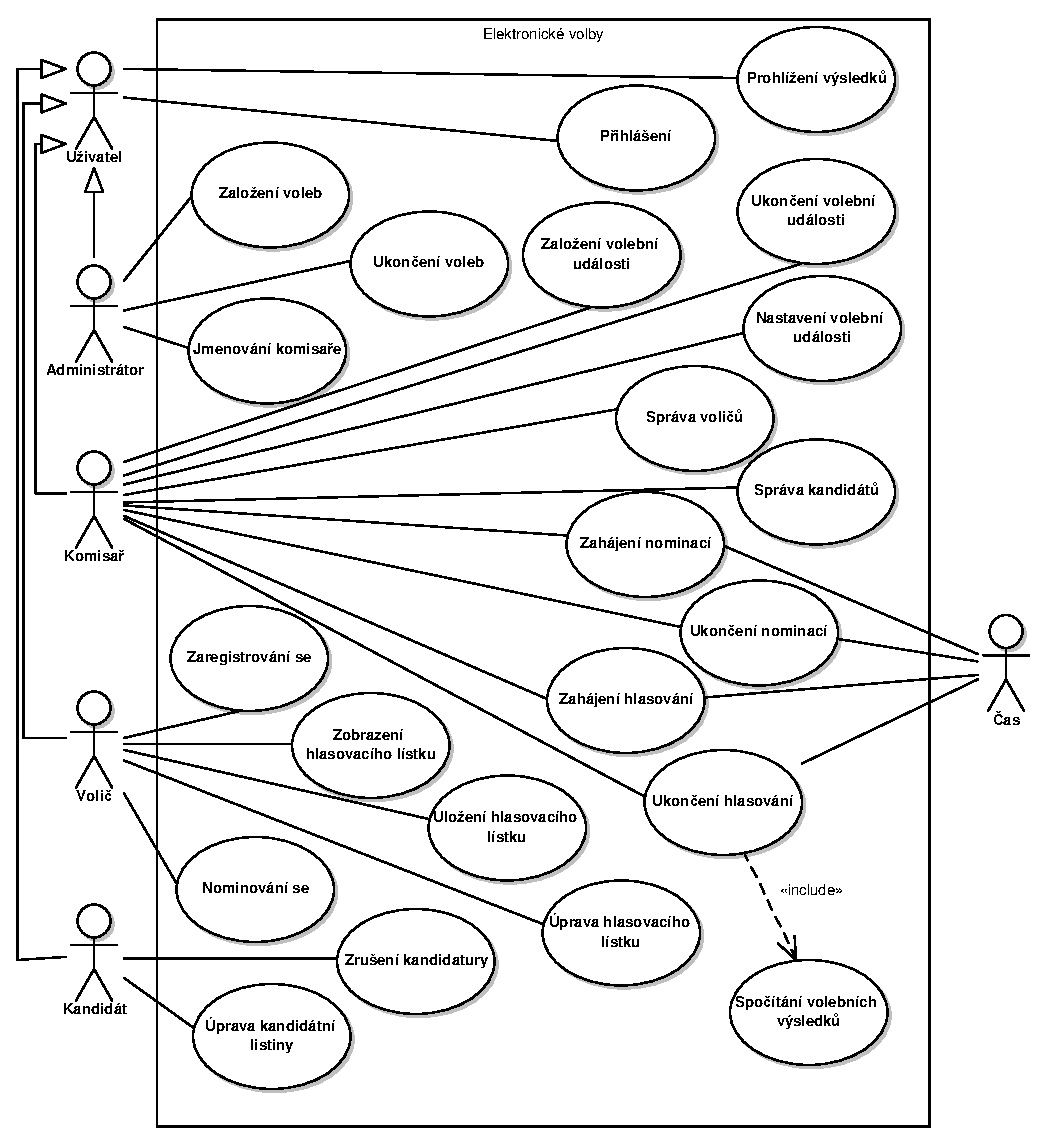
\includegraphics[scale=0.9]{diagrams/pripady_uziti.eps}
	\caption{Diagram případů užití.}
	\label{fig:pripady_uziti}
\end{figure}


\section{Technologie}

Při výběru technologií byly voleny open source či freeware řešení, které zajistí multiplatformnost systému.

\subsection{Server}

\subsubsection{Java EE}

Java Enterprise Edition je součást platformy Java určená pro vývoj podnikových aplikací a informačních systémů. Za jejím vývojem stojí společnost Sun Microsystems. Tuto technologii jsem zvolil pro její pokročilé možnosti a multiplatformní nasazení díky JVM.  Navíc prototyp eVoleb již byl napsán v Javě EE. Java EE vyžaduje ke svému běhu navíc aplikační server, jehož volba je popsána v kapitole \ref{aplikacni_server}. 

\subsubsection{Aplikační server} \label{aplikacni_server}

Prototyp eVoleb běžel na aplikačním serveru Glassfish 2.1.1. Tato verze již ovšem zastarává a je na ní problematické testování \cite{www:prototyp}. Proto jsem zvolil aplikační server Glassfish 3.1 \url{http://glassfish.java.net}, který přináší mnohá zlepšení. Glassfish jsem zvolil proto, že se jedná o referenční implementaci Javy EE6 přímo společností Sun Microsystems. Glassfish je open source projekt, ale existuje i jeho komerční verze, jenž se jmenuje Oracle Glassfish 3.1. Tyto dvě verze se od sebe v podstatě neliší, rozdíl je hlavně v podpoře a aktualizacích.

\subsubsection{Databáze}

Java EE disponuje sadou různých databázových konektorů díky technologii JDBC, které umožňují databázový stroj kdykoliv změnit. Při vývoji bude používána databáze MySQL \url{http://www.mysql.com}. Pro snadné nasazení je ale možné použití JavaDB, což je vestavěná databáze. Jedná se vlastně jen o knihovnu napsanou v jazyce Java a umožňuje přístup k datům uloženým na pevném disku za pomoci SQL dotazů.

\subsection{Klient}

\subsubsection{Java SE}

Java SE slouží k tvorbě desktopových aplikací, které běží pod JVM. Je tedy opět multiplatformní.

\subsection{Vývojové a testovací prostředí}

Vývoj probíhal na operačním systém Ubuntu 11.04 a bylo použito vývojové prostředí NetBeans IDE ve verzi 7.0. Jedná se o komplexní prostředí, které poskytuje snadnou správu kódu s integrací SVN pro verzování. Zároveň umožňuje ovládání aplikačního serveru Glassfish a napojení JDBC ovladačů na databázový stroj.

Pro testování webového prostředí posloužil webový prohlížeč Firefox 4.0.1.

\section{Snímač otisků prstů}

V kapitole \ref{sec:reserse_otisky} jsem rozebíral výhody a nevýhody jednotlivých technologií pro snímání otisků prstů. Pro vývoj klientské části, která má umožňovat autentizaci na základně otisku prstu, je třeba vybrat konkrétní snímač s kompatibilním SDK, které umožňuje práci s Javou. Využitím s biometrických údajů se zabývá mnoho společností a většina z nich nabízí i vlastní SDK určené právě pro jejich čtečky, což omezuje výběr. 

V úvahu je také třeba vzít ceny licencí SDK. V požadavcích v kapitole \ref{sec:obecne_pozadavky} je stanoveno, že budou využity open source či freeware technologie. Proto se klíčovým atributem pro výběr snímače otisků prstů stala cena licence SDK společně s podporou platformy Java. Při výběru jsem dbal i na to, aby SDK a snímače bylo možné používat pod operačními systémy MS Windows a Linux.

Pro detailnější prozkoumání jsem se zaměřil na produkty následujících společností, které nabízí jak samotné snímače otisků prstů, tak i k nim kompatibilní SDK.

\subsection{Griaule Biometrics}

Griaule Biometrics\footnote{\url{http://www.griaulebiometrics.com}} nabízí velmi robustní Fingerprint SDK s podporou více než 40 snímačů, ovšem při detailním zkoumání se ukázalo, že jejich verze SDK pro Javu má tento výběr omezen na zhruba čtvrtinové množství. 

SDK spolupracuje s mnoha platformami (C++ .NET, C\# .NET, Delphi 6-7, Visual Basic 6, VB .NET, ASP.net, Java, Java Applet) a je k dispozici i pro MS Windows i pro Linux. 

Dále v neprospěch tohoto SDK hovoří i licenční politika, která vyžaduje uhrazení licence pro každý vývojářský počítač, na kterém bude Fingerprint SDK nainstalováno. Cena jedné licence se pohybuje kolem \$100.

\subsection{Futronic}

Společnost Futronic\footnote{\url{http://www.futronic-tech.com}} vyvinula pro svůj snímač otisků prstů Futronic FS80 vlastní SDK, které podporuje MS Windows, Linux i MacOS a může se pochlubit spoluprací s platformami VB6, VC6, Borland Delphi, VB.NET a VC.NET, VB.2005, VC.2005 a samozřejmě Javou.

Bohužel toto SDK není veřejně dostupné a pro více informací či jeho získání je třeba kontaktovat přímo společnost Futronic. 

\subsection{Digital Persona}

Jako nejvhodnější se ukázalo SDK od společnosti Digital Persona\footnote{\url{http://www.digitalpersona.com}}, které je nabízeno jako freeware a k němuž je nabízen placený doplněk pro rychlejší porovnávání otisků prstů. Základní verze SDK však zcela postačuje, je k dispozici ve verzi pro MS Windows i pro Linux a spolupracuje s platformami Java, C, C++ a .NET.

Digital Persona k tomuto SDK nabízí i svůj vlastní snímač otisků prstů pod označením U.are.U 4500 Fingerprint Reader v ceně \$99.

\subsection{Vybrané SKD a snímač otisků prstů}

Pro vývoj jsem tedy zvolil SDK od společnosti Digital Persona a jejich snímač otisků prstů U.are.U 4500 Fingerprint Reader. Volba padle na něj především díky freewarovému SDK, které mají ostatní společnosti zpoplatněné, podpoře MS Windows a Linux a platformy Java.

%*****************************************************************************
\chapter{Návrh řešení a realizace}

Vzhledem k tomu, že systém vychází z prototypu eVolby, který již má své řešení navržené, budu v této práci popisovat jednotlivé iterace, ve kterých jsem ho modifikoval, přičemž v každé iteraci se zaměřím na problémy, se kterými jsme se setkal a popíši postup, kterým jsem se dopracoval k funkčnímu řešení. 

\section{První iterace} \label{sec:iterace:prvni}

\subsection{Cíl}

Jako první jsem si stanovil za cíl migraci z Glassfishe 2.0.1 na Glassfish verze 3.1. K tomuto rozhodnutí mě vedla hlavně podpora nejnovějších technologií Javy Enterprise Edition 6\footnote{\url{http://glassfish.java.net/public/comparing_v2_and_v3.html}}. S tím se pojí i možnost unit testů v EJB, jak uvádí i závěrečná zpráva z vývoje prototypu eVolby\cite{www:prototyp}.

\subsection{Postup}

\subsubsection{Sdílené knihovny}

Zatímco Glassfish 2.0.1 byl certifikován pro Java EE 5, jeho novější verze Glassfish 3.1 je již certifikována pro Java EE 6. S tím souvisí změna některých standardů, která měla na svědomí problémy při migraci. Zjistil jsem, že při deploy aplikace dochází k vyhazování chyby, že EJB moduly neobsahují žádné EJB. Bylo to způsobováno tím, že Glassfish vynechával ty EJB, ve kterých narazil na jakoukoliv chybu. Problém tkvěl ve sdílené knihovně POJO objektů, které slouží jako přepravní kontejnery mezi EJB moduly. Jakmile remote interface dané EJB obsahoval referenci na takový sdílený POJO objekt, Glassfish 3.1 zahlásil, že takový objekt nezná.

Takováto situace se dá řešit dvěma různými způsoby. První spočívá v umístění sdílené knihovny mezi knihovny přímo do Glassfishe. Já jsem zvolil druhý způsob, který je jednodušší na nasazení. A to, že jsem všechny tři EJB moduly spolu s webovým modulem zastřešil pod jednu Enterprise aplikaci, která se následně deployuje namísto každého modulu zvlášť. 

\subsubsection{Entity}

Dále se objevily chyby v definici entit, kdy některé entity neměly pojmenované joinovací sloupce. To způsobovalo nevygenerování tabulek do databáze.

\subsubsection{Databáze}

V původním návrhu je EJB modul Controller napojen na dvě databáze - první databáze obsahuje data o volebních událostech a druhá data o uživatelích systému. Jelikož uživatelská databáze měla pouze jednu tabulku, sloučil jsem tyto databáze do jedné, což vede k zjednodušení konfigurace při nasazení na server.

\subsection{Výstup}

Po skončení této iterace jsem měl funkční deploy pro Glassfish 3.1 využívající pouze tři databáze namísto čtyř s korektně vygenerovanými tabulkami.


\section{Druhá iterace}

\subsection{Cíl}

Druhým krokem bylo zprovoznění základní funkcionality a její otestování společně se zlepšením zabezpečení.

\subsection{Postup}

\subsubsection{Autentizační realm}

Původní projekt využíval pro autentizaci uživatelů file realm Glassfishe. Toto nicméně vedlo k duplikaci dat, neboť každý uživatel musel být jak v tomto file realmu, tak v databázi uživatelů. Nakonfiguroval jsem tedy v Glassfishi JDBC realm, který přes JNDI přistupuje do interní databáze uživatelů a zajišťuje jejich autentizaci na základě dat v uvedených tabulkách.

\subsubsection{JSF 2.0}

Jak již bylo zmíněno v první iteraci \ref{sec:iterace:prvni}, nová verze Glassfishe 3.1 s sebou přináší nejnovější technologie. To v sobě zahrnuje i přechod z JSF 1.2 na verzi JSF 2.0. Původní prototyp systému eVolby\cite{www:prototyp} využíval střídavě technologií JSP i tohoto zastaralého JSF.

Předělal jsem všechny webové stránky tak, aby jednotně používaly JSF 2.0 za využití systému šablon. Stránky tedy není neincludují hlavičku a patičku, jak tomu bylo původně, nýbrž využívají šablonovacího systému.

\subsubsection{Volební applet}

Applet napsaný v Javě FX se při testování prototypu systému eVolby\cite{www:prototyp} ukázal jako nepoužitelný. Hlavním problémem byla verze nainstalované Javy na klientském počítači, ke se applet spouštěl, společně s problematickou komunikací s hostitelským serverem.

Na doporučení ze závěrečné zprávy jsem tento applet z projektu vyřadil a nahradil ho klasickým formulářem. Ten zajišťuje mnohem pohodlnější, rychlejší a hlavně funkční hlasování.

\subsection{Výstup}

Na konci druhé iterace je projekt ve své základní funkční podobě, umožňuje snadnější přidávání uživatelů a bezproblémové hlasování.

\section{Třetí iterace}

\subsection{Cíl}

\subsection{Postup}

\subsection{Výstup}


%*****************************************************************************
\chapter{Testování}

\begin{itemize}
 \item Způsob, průběh a výsledky testování.
 \item Srovnání s existujícími řešeními, pokud jsou známy.
\end{itemize} 


%*****************************************************************************
\chapter{Závěr}

\begin{itemize}
\item Zhodnocení splnění cílů DP/BP a  vlastního přínosu práce (při formulaci je třeba vzít v potaz zadání práce).
\item Diskuse dalšího možného pokračování práce.
\end{itemize} 

%*****************************************************************************
% Seznam literatury je v samostatnem souboru reference.bib. Ten
% upravte dle vlastnich potreb, potom zpracujte (a do textu
% zapracujte) pomoci prikazu bibtex a nasledne pdflatex (nebo
% latex). Druhy z nich alespon 2x, aby se poresily odkazy.

% maximalizuje příjmení autora a špatně zvětšuje diakritiku

\bibliographystyle{abbrv}
%\bibliographystyle{csplainnat}
%\bibliographystyle{plain}
%\bibliographystyle{psc}
%\bibliographystyle{alpha}

\bibliography{reference}

%*****************************************************************************

\appendix

%*****************************************************************************
\chapter{Seznam použitých zkratek}

\begin{description}
\item[ČSÚ] Český statistický úřad
\item[ČTK] Česká tisková kancelář
\item[ČVUT] České vysoké učení technické v Praze
\item[DDoS] Distributed Denial of Service
\item[FAI] Fakulta aplikované informatiky
\item[FEL] Fakulta elektrotechnická
\item[FIT] Fakulta informačních technologií
\item[Java EE] Java Enterprise Edition
\item[Java SE] Java Standart Edition
\item[JDBC] Java Database Connectivity
\item[JSF] Java Server Faces
\item[JSP] Java Server Pages
\item[JVM] Java Virtual Machine
\item[HTTP] Hypertext Transfer Protocol
\item[HTTPS] Hypertext Transfer Protocol Secure
\item[IDE] Integrated Development Environment
\item[LDAP] Lightweight Directory Access Protocol
\item[POJO] Plain Old Java Object
\item[SDK] Software Development Kit
\item[SQL] Structured Query Language
\item[UML] Unified Modeling Language
\item[UTB] Univerzita Tomáše Bati ve Zlíně
\item[XML] eXtensible Markup Language
\item[Y36SI2] Řízení SW projektů 
\item[Y36SI3] Realizace programových systémů
\end{description}

%*****************************************************************************
\chapter{UML diagramy}
\textbf{\large Tato příloha není povinná a zřejmě se neobjeví v každé práci. Máte-li ale větší množství podobných diagramů popisujících systém, není nutné všechny umísťovat do hlavního textu, zvláště pokud by to snižovalo jeho čitelnost.}

%*****************************************************************************
\chapter{Instalační a uživatelská příručka}
\textbf{\large Tato příloha velmi žádoucí zejména u softwarových implementačních prací.}

%*****************************************************************************
\chapter{Obsah přiloženého CD}

\end{document}
